\XtoCBlock{AdaptivePT1}
\label{block:AdaptivePT1}
\begin{figure}[H]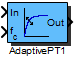
\includegraphics{AdaptivePT1}\end{figure} 

\begin{XtoCtabular}{Inports}
In & Input In(k)\tabularnewline
\hline
fc & Cutoff frequency\tabularnewline
\hline
\end{XtoCtabular}


\begin{XtoCtabular}{Outports}
Out & Output Out(k)\tabularnewline
\hline
\end{XtoCtabular}

\begin{XtoCtabular}{Mask Parameters}
V & Gain\tabularnewline
\hline
fmax & Maximum frequency [Hz]

(not used in floating point implementations)\tabularnewline
\hline
ts\_fact & Multiplication factor of base sampling time (in integer format)\tabularnewline
\hline
method & Discretization method\tabularnewline
\hline
\end{XtoCtabular}

\subsubsection*{Description:}
First order low pass with adaptive cut off frequency:

    G(s) = V/(s/(2*pi*fc) + 1)

% include optional documentation file
\InputIfFileExists{\XcHomePath/Library/Control/Doc/AdaptivePT1_Info.tex}{\vspace{1ex}}{}

\subsubsection*{Implementations:}
\begin{tabular}{l l}
\textbf{FiP8} & 8 Bit Fixed Point Implementation\tabularnewline
\textbf{FiP16} & 16 Bit Fixed Point Implementation\tabularnewline
\textbf{FiP32} & 32 Bit Fixed Point Implementation\tabularnewline
\textbf{Float32} & 32 Bit Floating Point Implementation\tabularnewline
\textbf{Float64} & 64 Bit Floating Point Implementation\tabularnewline
\end{tabular}

\XtoCImplementation{FiP8}
\index{Block ID!3408}
\nopagebreak[0]
% Implementation details
\begin{tabular}{l l}
\textbf{Name} & FiP8 \tabularnewline
\textbf{ID} & 3408 \tabularnewline
\textbf{Revision} & 0.1 \tabularnewline
\textbf{C filename} & AdaptivePT1\_FiP8.c \tabularnewline
\textbf{H filename} & AdaptivePT1\_FiP8.h \tabularnewline
\end{tabular}
\vspace{1ex}

8 Bit Fixed Point Implementation

\begin{XtoCtabular}{Controller Parameters}
w\_scale & Calculation base for wc: -2*pi*Ts*fmax\tabularnewline
\hline
gain & Gain\tabularnewline
\hline
sfr & Shift factor for gain\tabularnewline
\hline
in\_old & In(k-1)\tabularnewline
\hline
\end{XtoCtabular}

% Implementation data structure
\XtoCDataStruct{Data Structure:}
\begin{lstlisting}
typedef struct {
     uint16        ID;
     int8          *In;
     int8          *fc;
     int8          Out;
     int8          w_scale;
     int8          gain;
     uint8         sfr;
     int8          in_old;
} ADAPTIVEPT1_FIP8;
\end{lstlisting}

\ifdefined \AddTestReports
\InputIfFileExists{\XcHomePath/Library/Control/Doc/Test_AdaptivePT1_FiP8.tex}{}{}
\fi
\XtoCImplementation{FiP16}
\index{Block ID!3409}
\nopagebreak[0]
% Implementation details
\begin{tabular}{l l}
\textbf{Name} & FiP16 \tabularnewline
\textbf{ID} & 3409 \tabularnewline
\textbf{Revision} & 1 \tabularnewline
\textbf{C filename} & AdaptivePT1\_FiP16.c \tabularnewline
\textbf{H filename} & AdaptivePT1\_FiP16.h \tabularnewline
\end{tabular}
\vspace{1ex}

16 Bit Fixed Point Implementation

\begin{XtoCtabular}{Controller Parameters}
w\_scale & Calculation base for wc: -2*pi*Ts*fmax\tabularnewline
\hline
gain & Gain\tabularnewline
\hline
sfr & Shift factor for gain\tabularnewline
\hline
in\_old & In(k-1)\tabularnewline
\hline
\end{XtoCtabular}

% Implementation data structure
\XtoCDataStruct{Data Structure:}
\begin{lstlisting}
typedef struct {
     uint16        ID;
     int16         *In;
     int16         *fc;
     int16         Out;
     int16         w_scale;
     int16         gain;
     uint8         sfr;
     int16         in_old;
} ADAPTIVEPT1_FIP16;
\end{lstlisting}

\ifdefined \AddTestReports
\InputIfFileExists{\XcHomePath/Library/Control/Doc/Test_AdaptivePT1_FiP16.tex}{}{}
\fi
\XtoCImplementation{FiP32}
\index{Block ID!3410}
\nopagebreak[0]
% Implementation details
\begin{tabular}{l l}
\textbf{Name} & FiP32 \tabularnewline
\textbf{ID} & 3410 \tabularnewline
\textbf{Revision} & 0.1 \tabularnewline
\textbf{C filename} & AdaptivePT1\_FiP32.c \tabularnewline
\textbf{H filename} & AdaptivePT1\_FiP32.h \tabularnewline
\end{tabular}
\vspace{1ex}

32 Bit Fixed Point Implementation

\begin{XtoCtabular}{Controller Parameters}
w\_scale & Calculation base for wc: -2*pi*Ts*fmax\tabularnewline
\hline
gain & Gain\tabularnewline
\hline
sfr & Shift factor forgain\tabularnewline
\hline
in\_old & In(k-1)\tabularnewline
\hline
\end{XtoCtabular}

% Implementation data structure
\XtoCDataStruct{Data Structure:}
\begin{lstlisting}
typedef struct {
     uint16        ID;
     int32         *In;
     int32         *fc;
     int32         Out;
     int32         w_scale;
     int32         gain;
     uint8         sfr;
     int32         in_old;
} ADAPTIVEPT1_FIP32;
\end{lstlisting}

\ifdefined \AddTestReports
\InputIfFileExists{\XcHomePath/Library/Control/Doc/Test_AdaptivePT1_FiP32.tex}{}{}
\fi
\XtoCImplementation{Float32}
\index{Block ID!3411}
\nopagebreak[0]
% Implementation details
\begin{tabular}{l l}
\textbf{Name} & Float32 \tabularnewline
\textbf{ID} & 3411 \tabularnewline
\textbf{Revision} & 0.1 \tabularnewline
\textbf{C filename} & AdaptivePT1\_Float32.c \tabularnewline
\textbf{H filename} & AdaptivePT1\_Float32.h \tabularnewline
\end{tabular}
\vspace{1ex}

32 Bit Floating Point Implementation

\begin{XtoCtabular}{Controller Parameters}
w\_scale & Calculation base for wc: -2*pi*Ts*fmax\tabularnewline
\hline
gain & Gain\tabularnewline
\hline
in\_old & In(k-1)\tabularnewline
\hline
\end{XtoCtabular}

% Implementation data structure
\XtoCDataStruct{Data Structure:}
\begin{lstlisting}
typedef struct {
     uint16        ID;
     float32       *In;
     float32       *fc;
     float32       Out;
     float32       w_scale;
     float32       gain;
     float32       in_old;
} ADAPTIVEPT1_FLOAT32;
\end{lstlisting}

\ifdefined \AddTestReports
\InputIfFileExists{\XcHomePath/Library/Control/Doc/Test_AdaptivePT1_Float32.tex}{}{}
\fi
\XtoCImplementation{Float64}
\index{Block ID!3412}
\nopagebreak[0]
% Implementation details
\begin{tabular}{l l}
\textbf{Name} & Float64 \tabularnewline
\textbf{ID} & 3412 \tabularnewline
\textbf{Revision} & 0.1 \tabularnewline
\textbf{C filename} & AdaptivePT1\_Float64.c \tabularnewline
\textbf{H filename} & AdaptivePT1\_Float64.h \tabularnewline
\end{tabular}
\vspace{1ex}

64 Bit Floating Point Implementation

\begin{XtoCtabular}{Controller Parameters}
w\_scale & Calculation base for wc: -2*pi*Ts*fmax\tabularnewline
\hline
gain & Gain\tabularnewline
\hline
in\_old & In(k-1)\tabularnewline
\hline
\end{XtoCtabular}

% Implementation data structure
\XtoCDataStruct{Data Structure:}
\begin{lstlisting}
typedef struct {
     uint16        ID;
     float64       *In;
     float64       *fc;
     float64       Out;
     float64       w_scale;
     float64       gain;
     float64       in_old;
} ADAPTIVEPT1_FLOAT64;
\end{lstlisting}

\ifdefined \AddTestReports
\InputIfFileExists{\XcHomePath/Library/Control/Doc/Test_AdaptivePT1_Float64.tex}{}{}
\fi
